Generativní modely využívající latentních proměnných umožňují transformaci dat
do \emph{jednodušších} a lépe interpretovatelných latentních prostorů.
A tím pádem umožňují taková data lépe prozkoumat a porozumět jim. \cite{Kingma2019}

Přidruženým odvětvím aplikacím hlubokých generativních modelů je syntéza přijatelných pseudo-dat s určitou sadou chtěných vlastností, často také nazývána \emph{umělá kreativita} (artificial creativity).


\newpage
\section{Generativní modelování obrazových dat}
Generativní modelování přirozených obrázků představuje jednu z nejaktuálnějších úloh učení bez učitele vůbec. \cite{Gulrajani2016}
VAE (a jeho rozšíření) natrénované na datasetech obrazových dat v této oblasti dosahují excelentních výsledků.
DRAW (rozšíření VAE, viz \autoref{sec:draw}) je jedna z vůbec prvních architektur VAE modifikovaná k generování \textbf{zcela nových a realistických obrázků}, jenž nebyly součástí trénovací množiny.
\begin{figure}[H]
    \centering
    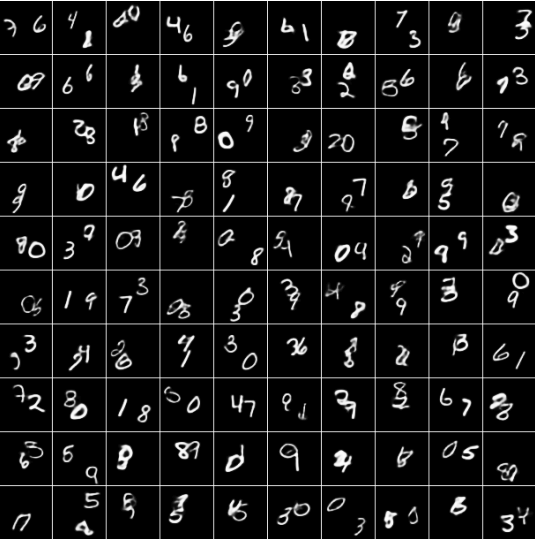
\includegraphics[width=0.55\textwidth]{figures/applications/mnist_double_digits_gregor.png}
    \caption{Aplikace VAE na generování zcela nových obrázků dvou cifer, trénováno na MNIST datasetu. Převzato z \cite{Gregor2015}.}
    \label{fig:mnist_double_digits_gregor}
\end{figure}

Další rozšířenou architekturou je PixelVAE \cite{Gulrajani2016}, která oproti DRAW nabízí větší kvalitu realistických obrázků vzorkovaných z generativního modelu.

\begin{figure}[H]
    \centering
    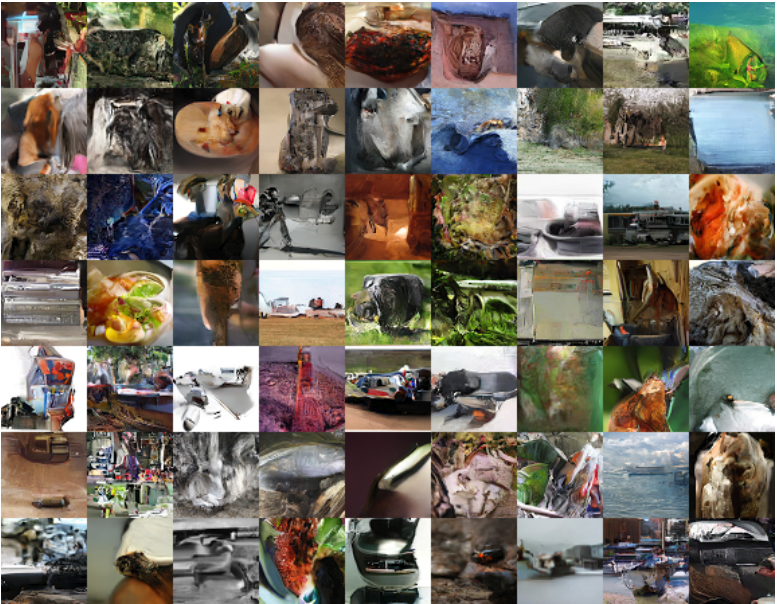
\includegraphics[width=0.55\textwidth]{figures/applications/image_net_pixel_vae_gulrajani.png}
    \caption{Výsledek vzorkování PixelVAE \cite{Gulrajani2016}.}
    \label{fig:image_net_pixel_vae_gulrajani}
\end{figure}

\newpage
\section{Opakovana syntéza obrazových dat}
Populární aplikací VAE je (re)syntéza obrazových dat.
Využití jednoduchého modelu VAE k opakované syntéze obrazových dat (konkrétně snímků lidských obličejů) představuje \cite{White2016}.

VAE lze optimalizovat za účelem zformování generativního modelu skrze vstupní sadu obrazových dat.
Z takového generativního modelu pak lze vzorkovat zcela nové obrázky, které nebyly součástí trénovací množiny dat. \cite{Kingma2019}

\begin{figure}[H]
    \centering
    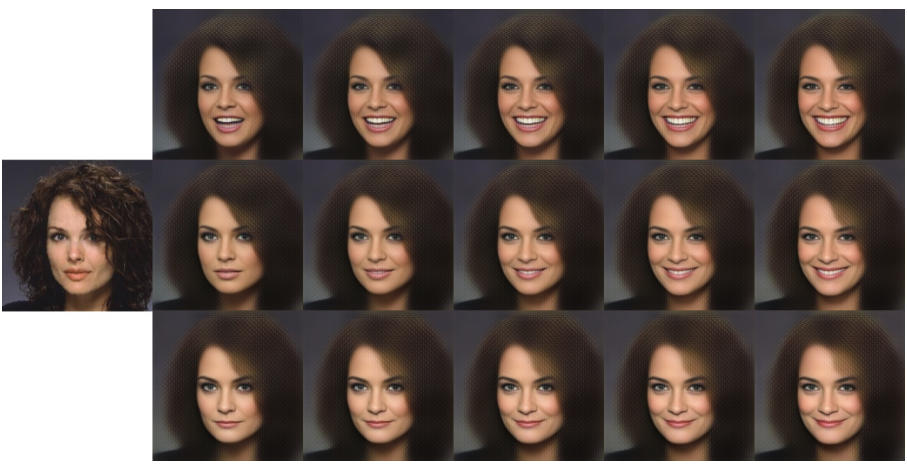
\includegraphics[width=0.9\textwidth]{figures/applications/vae_smile_vector_white.png}
    \caption{Využití VAE pro opakovanou syntézu vstupního obrázku. V tomto příkladě lze pozorovat posun původního obrázku (vlevo) v modifikovaném latentním prostoru ve směru \emph{vektoru úsměvu}, což má za výsledek progresivně více usmívající se obličej. Převzato z \cite{White2016}.}
    \label{fig:vae_smile_vector_white}
\end{figure}


\textbf{Takto naučený model ale nabízí ještě jednu zajímavou aplikaci}.
Inferenční model (enkodér) totiž umožňuje zakódovat reálné obrázky do jeho latentního prostoru.
Tento kód pak lze ve vzniklém latentní prostoru modifikovat a následně jej dekódovat zpět do pozorovaného prostoru.
Aplikace jednoduchých transformací – například pouhé lineární transformace – na tento prostor má často za důsledek \textbf{sémanticky významnou modifikaci původního obrázku}.
\autoref{fig:vae_smile_vector_white} demonstruje modifikaci obrázku obličeje v latentním prostoru podél \textbf{"vektoru úsměvu"}, což činí původní obrázek progresivně více veselejším (lze pozorovat i osu \emph{otevřených úst} při úsměvu). \cite{Kingma2019}

\newpage
\section{Predikce barvy pixelů černobílých obrázků}
Další slibnou aplikací VAE v oblasti generativního modelování obrazových dat je predikce původní barvy jednotlivých pixelů obrázku na základě černobílého (\emph{grayscale}) vstupu.

V \cite{Deshpande2017} autoři představují architekturu VAE, která rozšiřuje CVAE a modifikuje jeho ztrátovou funkci (a to za účelem zpřesnění predikce barvy pixelů a vyhnutí se rozostřeným vygenerovaným vzorkům).
\begin{figure}[H]
    \centering
    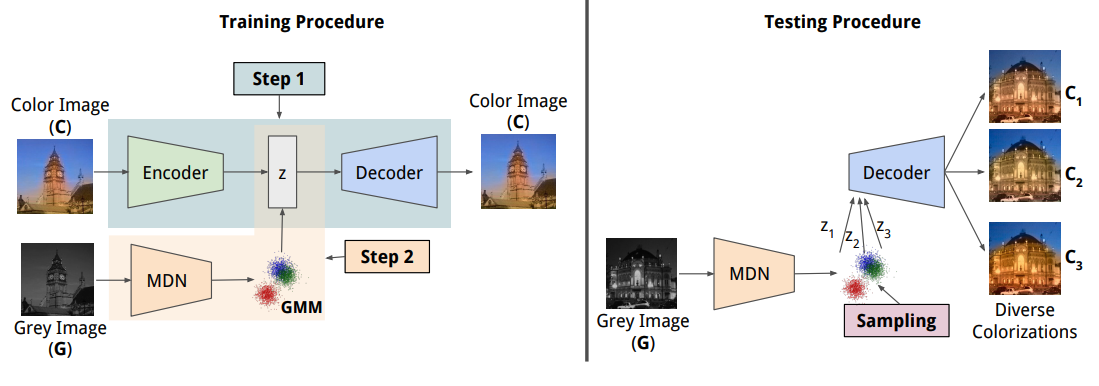
\includegraphics[width=0.9\textwidth]{figures/applications/predicting_pixel_colors_deshpande_vae_schema.png}
    \caption{Schema trénovací a vzorkovací procedury rozšířeného CVAE pro predikci barvy pixelů původního obrázku. Převzato z \cite{Deshpande2017}.}
    \label{fig:predicting_pixel_colors_deshpande_schema}
\end{figure}

V trénovací fázi se jako první model naučí nízkodimenzionální reprezentaci $z$ pro barevné pole $C$.
Poté je natrénován podmíněný pravděpodobnostní model $P(z \mid G)$, který generuje nízkodimenzionální reprezentaci na základě černobílého vstupu $G$. 
Tento pravděpodobnostní model lze poté vzorkovat a využít dekoder modul vzniklého VAE pro vygenerování rozmanitých barevných polí původního obrázku na výstupu (tj. vygenerování více kombinací \emph{obarvení} grayscale obrázku).
\textbf{Při vzorkování generativní model jako vstup obdrží pouze grayscale obrázek}. Schéma procedur tohoto modelu zachycuje \autoref{fig:predicting_pixel_colors_deshpande_schema}. \cite{Deshpande2017}

\begin{figure}[H]
    \centering
    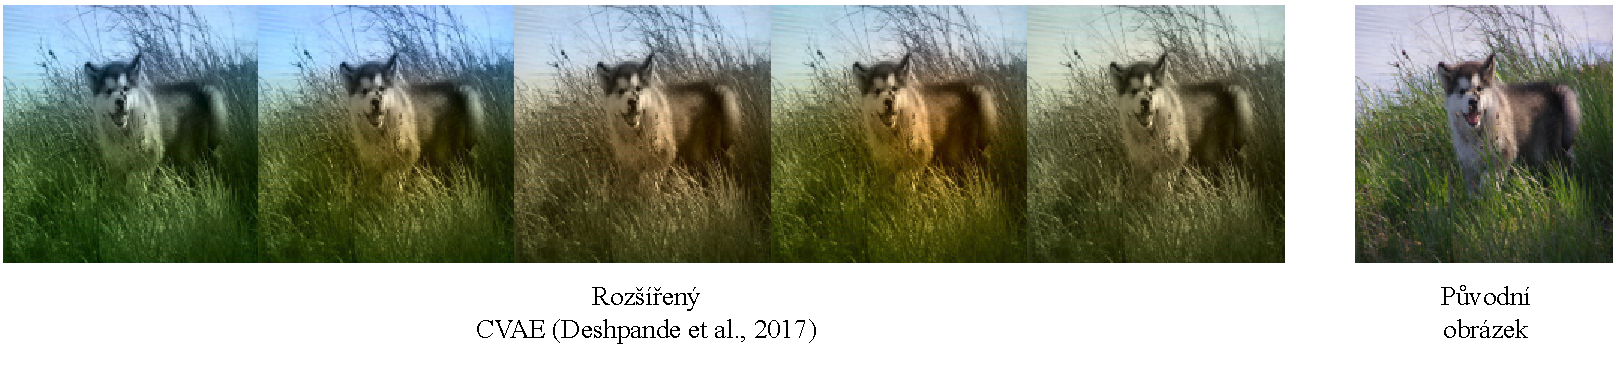
\includegraphics[width=0.9\textwidth]{figures/applications/predicting_pixel_colors_deshpande.pdf}
    \caption{Vzorek vygenerovaných variací (vlevo) obarvení původního obrázku (vpravo). Vstupem pro generativní model byl pouze černobílý obrázek. Převzato z \cite{Deshpande2017}.}
    \label{fig:predicting_pixel_colors_deshpande}
\end{figure}

\autoref{fig:predicting_pixel_colors_deshpande} prezentuje vzniklé variace obarvení původního obrázku na základě černobílého vstupu.
Takto naučený model tedy lze využít například k obarvení černobílých fotografií.

\newpage
\section{Rekonstrukce obrazových dat}

\newpage
\section{Komprese}

\newpage
\section{Syntéza přirozeného jazyka}
Jednu možnou aplikací VAE na úlohu syntézy přirozené jazyka, konkrétně \textbf{interpolace vět} představuje \cite{Bowman2016}.

Zde je jednoduchý VAE (se stejnou strukturou, jakou prezentuje \autoref{chap:vae}) trénován na korpusu přirozeného anglického jazyka.

\begin{figure}[H]
    \centering
    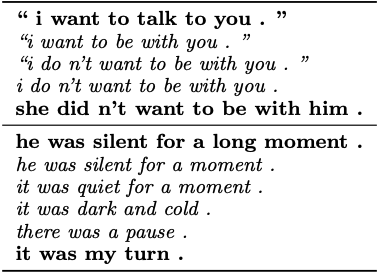
\includegraphics[width=0.9\textwidth]{figures/applications/vae_sentence_interpolation_bowman.png}
    \caption{Aplikace VAE pro interpolaci přirozeného jazyka mezi dvojicí vět. Vstupní páry vět jsou vyznačeny tučně, přechodné věty vygenerované modelem VAE jsou kurzívou.
    Pozoruhodně jsou přechodné věty \textbf{gramaticky správné}, drží \textbf{syntaktickou správnost} a \textbf{zachovávají tématický kontext} vstupních párů vět. Převzato z \cite{Bowman2016}.}
    \label{fig:vae_sentence_interpolation_bowman}
\end{figure}

Výsledkem je model, jenž je schopen úspěšně \textbf{interpolovat mezi větami} a \textbf{doplnit do vět chybějící slova}. \autoref{fig:vae_sentence_interpolation_bowman} prezentuje schopnost takto naučeného modelu k interpolaci mezi vstupními páry vět. \cite{Bowman2016}

\newpage
\section{Návrh chemikálií}
Doposud byly prezentovány spíše triviální využití VAE.
Nicméně jedna z nedávných aplikací VAE k vědeckým účelům je popsána v \cite{GomezBombarelli2018}.
V této publikaci je jednoduchý VAE (se strukturou modulů, které popisuje \autoref{chap:vae}) trénován na datové sadě obsahující stovky tisíc existujících chemických struktur.
Jejich výsledný latentní prostor (a jeho spojitá reprezentace) je posléze použit k gradientní optimalizaci určitých vlastností celkového modelu.
Princip této metody k návrhu molekul léků (či alespoň jejich přidružených molekul) demonstruje \autoref{fig:vae_molecule_design_gomez}. \cite{Kingma2019}

\begin{figure}[H]
    \centering
    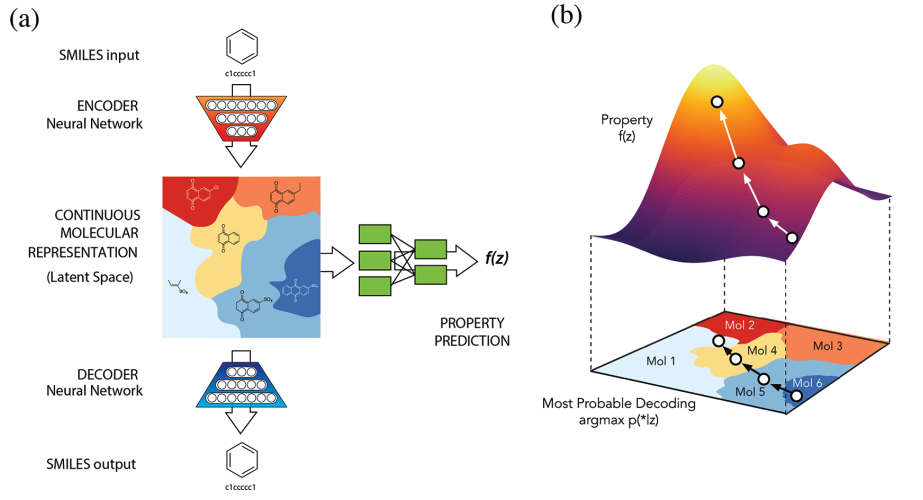
\includegraphics[width=0.9\textwidth]{figures/applications/vae_molecule_design_gomez.png}
    \caption{Aplikace VAE k návrhu chemikálií. Obrázek (a): Proces naučení latentní spojitá reprezentace molekul $z$ z velkého vstupního datasetu. Obrázek (b): Takto naučená spojitá reprezentace umožňuje hledání nových molekul které maximalizují $f(z)$ (určitou \emph{chtěnou} vlastnost molekul). Převzato z \cite{GomezBombarelli2018}.}
    \label{fig:vae_molecule_design_gomez}
\end{figure}

\newpage
\section{Astronomie}
Další aplikací VAE v oblasti vědy prezentuje \cite{Ravanbakhsh2016}.
V této studii jsou VAE aplikovány k simulaci pozorování vzdálených galaxií.
Vzorky generované VAE pomáhají kalibrovat systémy, jejichž úkolem je detekovat \emph{zkreslení} (shearing) pozorování vzdálených galaxií, které je způsobeno slabým jevem gravitační čočky
\footnote{Pojem gravitační čočky vychází ze spojné (optické) čočky. Užívá se pro popis objektu (např. klastru galaxií), který vlivem svého gravitačního pole způsobuje prohnutí paprsků světla vycházejících ze zdroje směrem k pozorovateli.},
vlivem přítomnosti temné hmoty mezi Zemí a těmito (pozorovanými) galaxiemi. \cite{Kingma2019}

\begin{figure}[H]
    \centering
    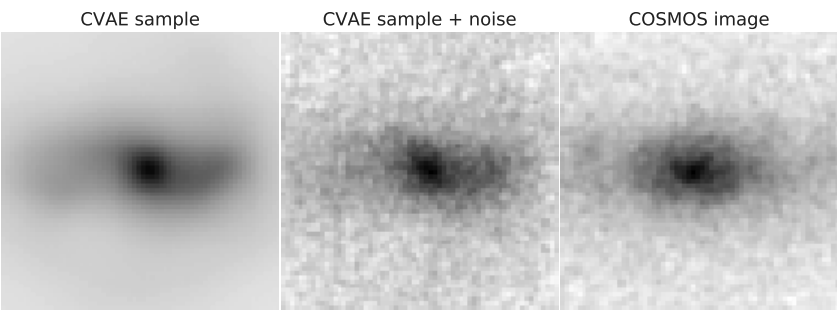
\includegraphics[width=0.9\textwidth]{figures/applications/vae_space_pseudodata_ravanbakhsh.png}
    \caption{Aplikace VAE k generování syntetických pseudo dat využitelných pro kalibraci systému k detekci zkreslení pozorování vzdálených galaxií. K vygenerovanému vzorku pozorování je dodatečně přidán šum. Levý obrázek představuje vzorek z generativního modelu, pravý obrázek představuje reálný snímek pozorování. Převzato z \cite{Ravanbakhsh2016}.}
    \label{fig:vae_space_pseudodata_ravanbakhsh}
\end{figure}


Vzhledem k tomu, že jev gravitační čočky je slabý, je nutné tyto systémy kalibrovat s \textbf{realistickými} obrázky s odpovídajícím množství zkreslení.
A vzhledem k tomu, že dostupné \textbf{množství} takových \textbf{reálných dat je aktuálně velmi omezené}, přistoupili autoři studie k využití VAE (respektive CVAE, viz \autoref{sec:cvae}) za účelem \textbf{syntézy pseudo-dat}, které jsou následně pro kalibraci využity. Jeden takový vzorek prezentuje \autoref{fig:vae_space_pseudodata_ravanbakhsh}.